% This work is licensed under the Creative Commons
% Attribution-NonCommercial-ShareAlike 4.0 International License. To view a copy
% of this license, visit http://creativecommons.org/licenses/by-nc-sa/4.0/ or
% send a letter to Creative Commons, PO Box 1866, Mountain View, CA 94042, USA.

\tikzset{every picture/.style={line width=0.75pt}} %set default line width to 0.75pt        

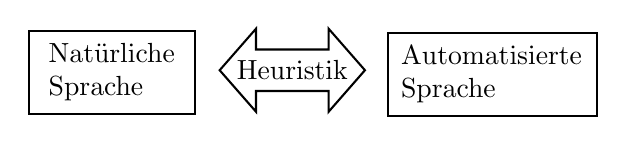
\begin{tikzpicture}[x=0.75pt,y=0.75pt,yscale=-1,xscale=1]
%uncomment if require: \path (0,300); %set diagram left start at 0, and has height of 300

%Shape: Rectangle [id:dp02241090211127661] 
\draw   (81,126) -- (161,126) -- (161,166) -- (81,166) -- cycle ;
%Shape: Rectangle [id:dp20165869726734287] 
\draw   (254,127) -- (355,127) -- (355,167) -- (254,167) -- cycle ;
%Left Right Arrow [id:dp33351638469477385] 
\draw   (173,145) -- (190.5,125) -- (190.5,135) -- (225.5,135) -- (225.5,125) -- (243,145) -- (225.5,165) -- (225.5,155) -- (190.5,155) -- (190.5,165) -- cycle ;

% Text Node
\draw (121,146) node  [align=left] {Natürliche\\Sprache};
% Text Node
\draw (304,147) node  [align=left] {Automatisierte\\Sprache};
% Text Node
\draw (208,145) node  [align=left] {Heuristik};


\end{tikzpicture}